\section{Results}
\begin{paracol}
    {2}
    This section covers the observed characteristics of the implemented coverage planners, perception methods and solutions regarding manipulation. 
    \subsection{Coverage Planners}
    Two path planners have been assessed and compared:
    \begin{itemize}
    \item Morphology-based Skeleton Coverage
    \item Spanning Tree coverage
    \end{itemize}
    
    The morphology-based skeleton coverage planner (Figure \ref{fig_skeletonpathresult}) performed well in laboratory-like environments but worse in larger open spaces. The planner allowed the robot to maneuver efficiently in between objects such as tables and chairs, while still being able to pass through narrow straights. This particular planner also resulted in the least amount of sharp turns which, due to the simple nature of the MIRTE Master's odometry (wheel encoders only), helped the robot to not lose track of where it was and thus keep the map clean and minimise drift. However, the skeleton planner performed slightly worse in terms of coverage performance. This is due to the lower density of the planned path, which resulted in the robot sometimes missing the edges of the free space that needs to be scanned for objects.
    
    \begin{figure}[H]
    \centering
    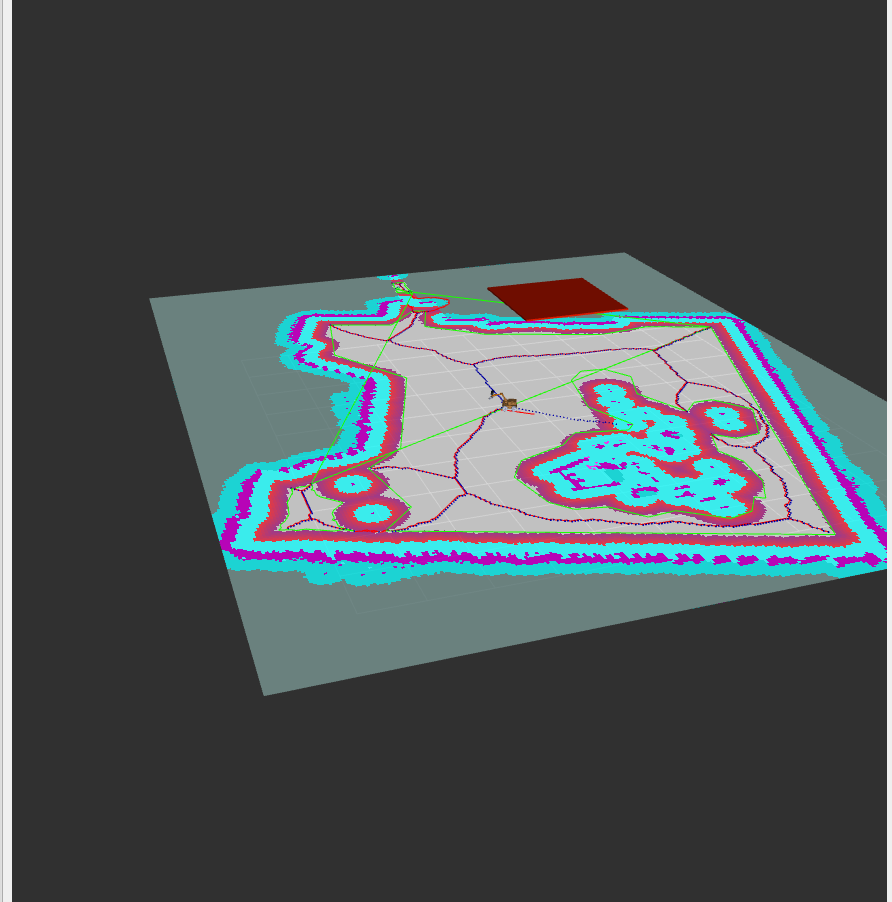
\includegraphics[width=0.99\linewidth]{latex/figures/SkeletonMapRviz.png}
    \caption{Skeleton path in laboratory environment}
    \label{fig_skeletonpathresult}
    \end{figure}
    \syncallcounters
    \switchcolumn
    
    The spanning tree coverage planner performed well in large open spaces, but unlike the morphology based skeleton coverage planner, it struggled more with planning paths in tighter spaces such as laboratory environments (see Figure \ref{fig_spanningtreeresults} in the top right), resulting in separate path loops being stitched together and occasionally missing narrow spots between the loops. Also, due to the nature of the coverage pattern, a lot of turns with a tight radius are generated which resulted in the robot sometimes slowly accumulating drift in the odometry, resulting in a less accurate map and unreliable localisation.
    
    \begin{figure}[H]
    \centering
    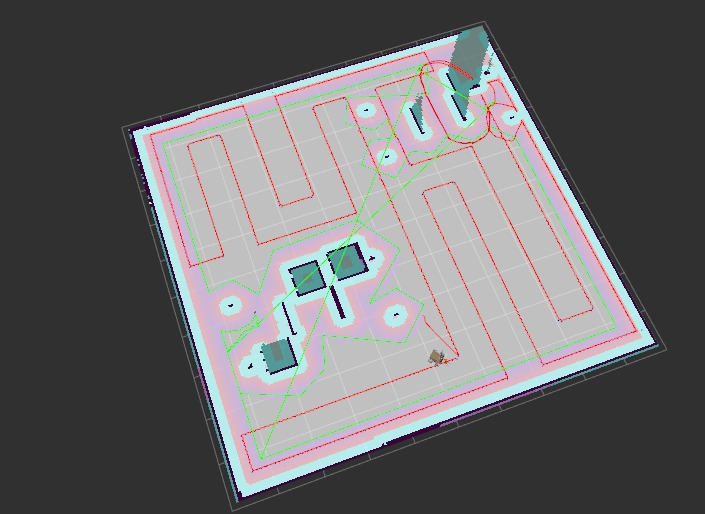
\includegraphics[width=0.99\linewidth]{latex/figures/SpanningTreeResult.jpeg}
    \caption{Spanning tree path in laboratory environment}
    \label{fig_spanningtreeresults}
    \end{figure}

    \subsection{Object Localization and Classification}
     For object detection worked on a localization method and a classification method. Our object localizator relies on bounding boxes that are retrieved from pointclouds made by the depthcamera's depth images. Our object detector was able to find objects sized within 1\textit{cm} to 6\textit{cm}. A bounding box drawn around a found object in the pointcloud is shown in the figure below. The custom-made YOLO26 object detection model worked as intended, being able to  classify the localized objects correctly. In the figure shown below a frame from the RGB sensor of the depth camera is shown in the bottom right corner.
    \end{paracol}
    \newpage
    \begin{paracol}
        {2}
    \begin{figure}[H]
    \centering
    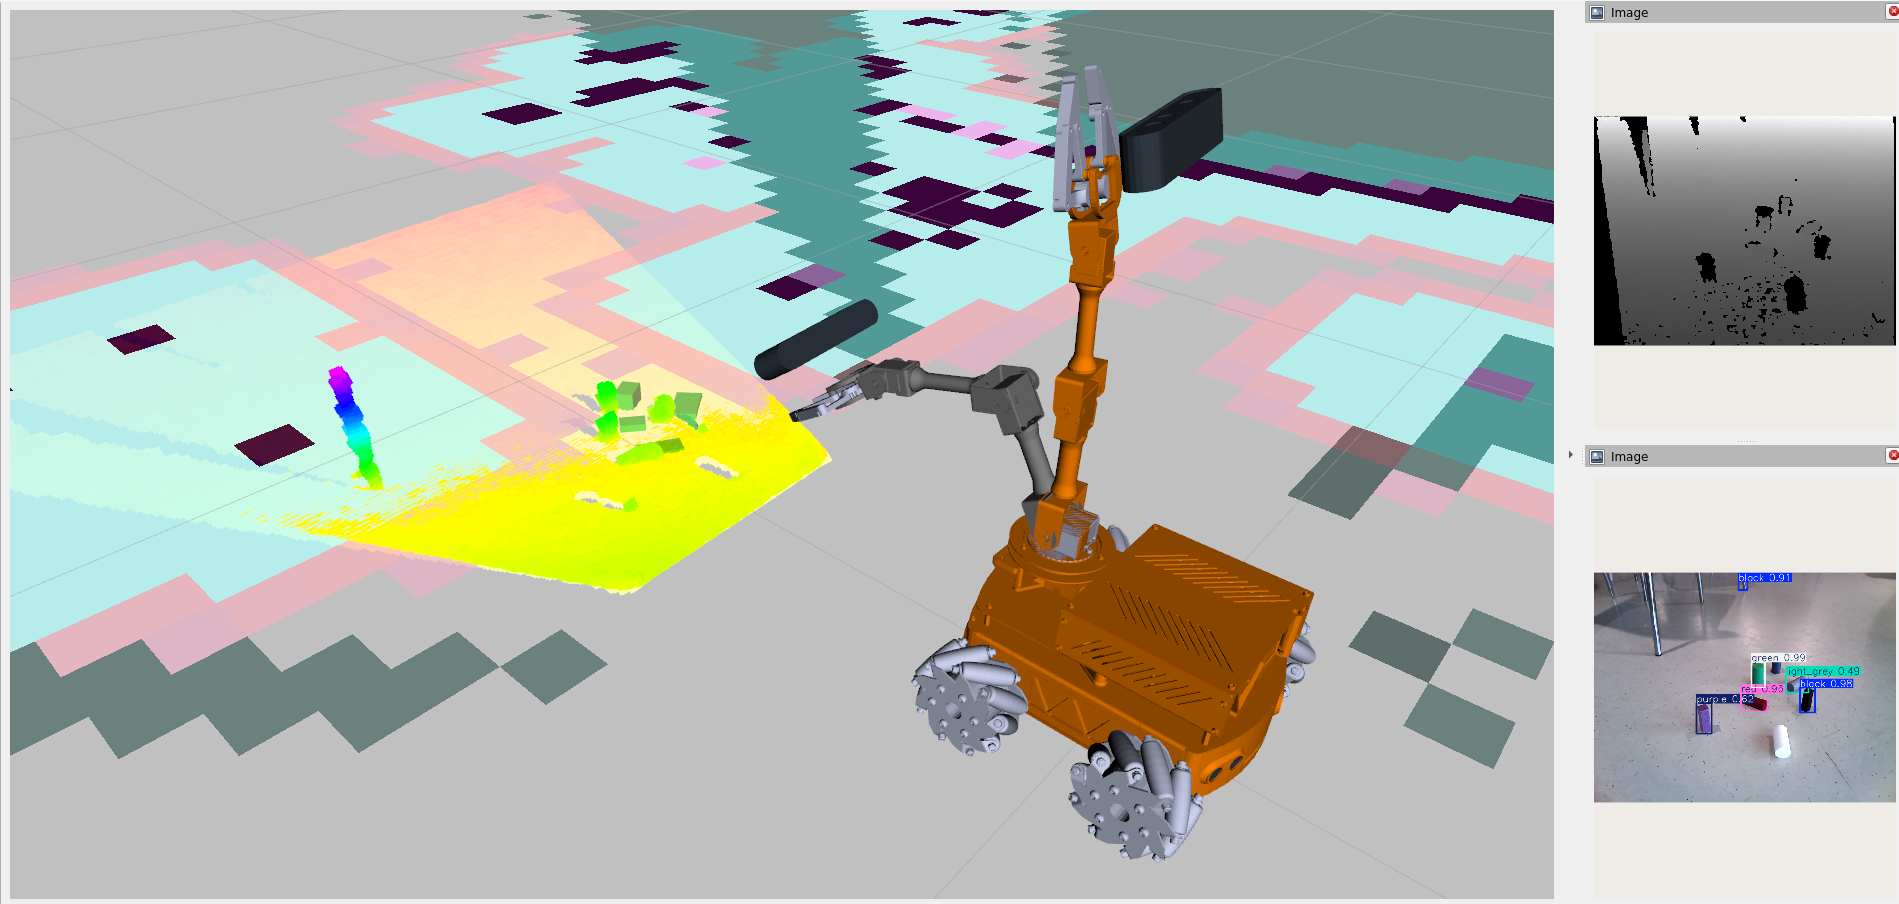
\includegraphics[width=0.99\linewidth]{latex/figures/BoundingBoxYolo.png}
    \caption{Bounding box drawn around found objects (center) and YOLO26 working simultaneously (bottom right).}
    \label{fig_boundingboxesandyolo}
    \end{figure}
    
    \subsection{Manipulation}
    \paragraph{Movement accuracy}
    The manipulation of the actuator has seen major improvements regarding movement accuracy. The initial accuracy of the actuator was around 15\textit{cm}. After reworking the code, the actuator was controlled by a function that did not rely on joint approximation. This reduced the error significantly, resulting in a theoretical movement error of just 1\textit{mm}.

    \paragraph{Gripping performance}
    The gripping performance of the original robot was slightly increased by adding rubberized patches to gripping surfaces to the gripper. This has helped gripping the smooth, plastic testing objects when the gripper approached the objects at a sub-optimal angle of approach.
    \begin{figure}[H]
    \centering
    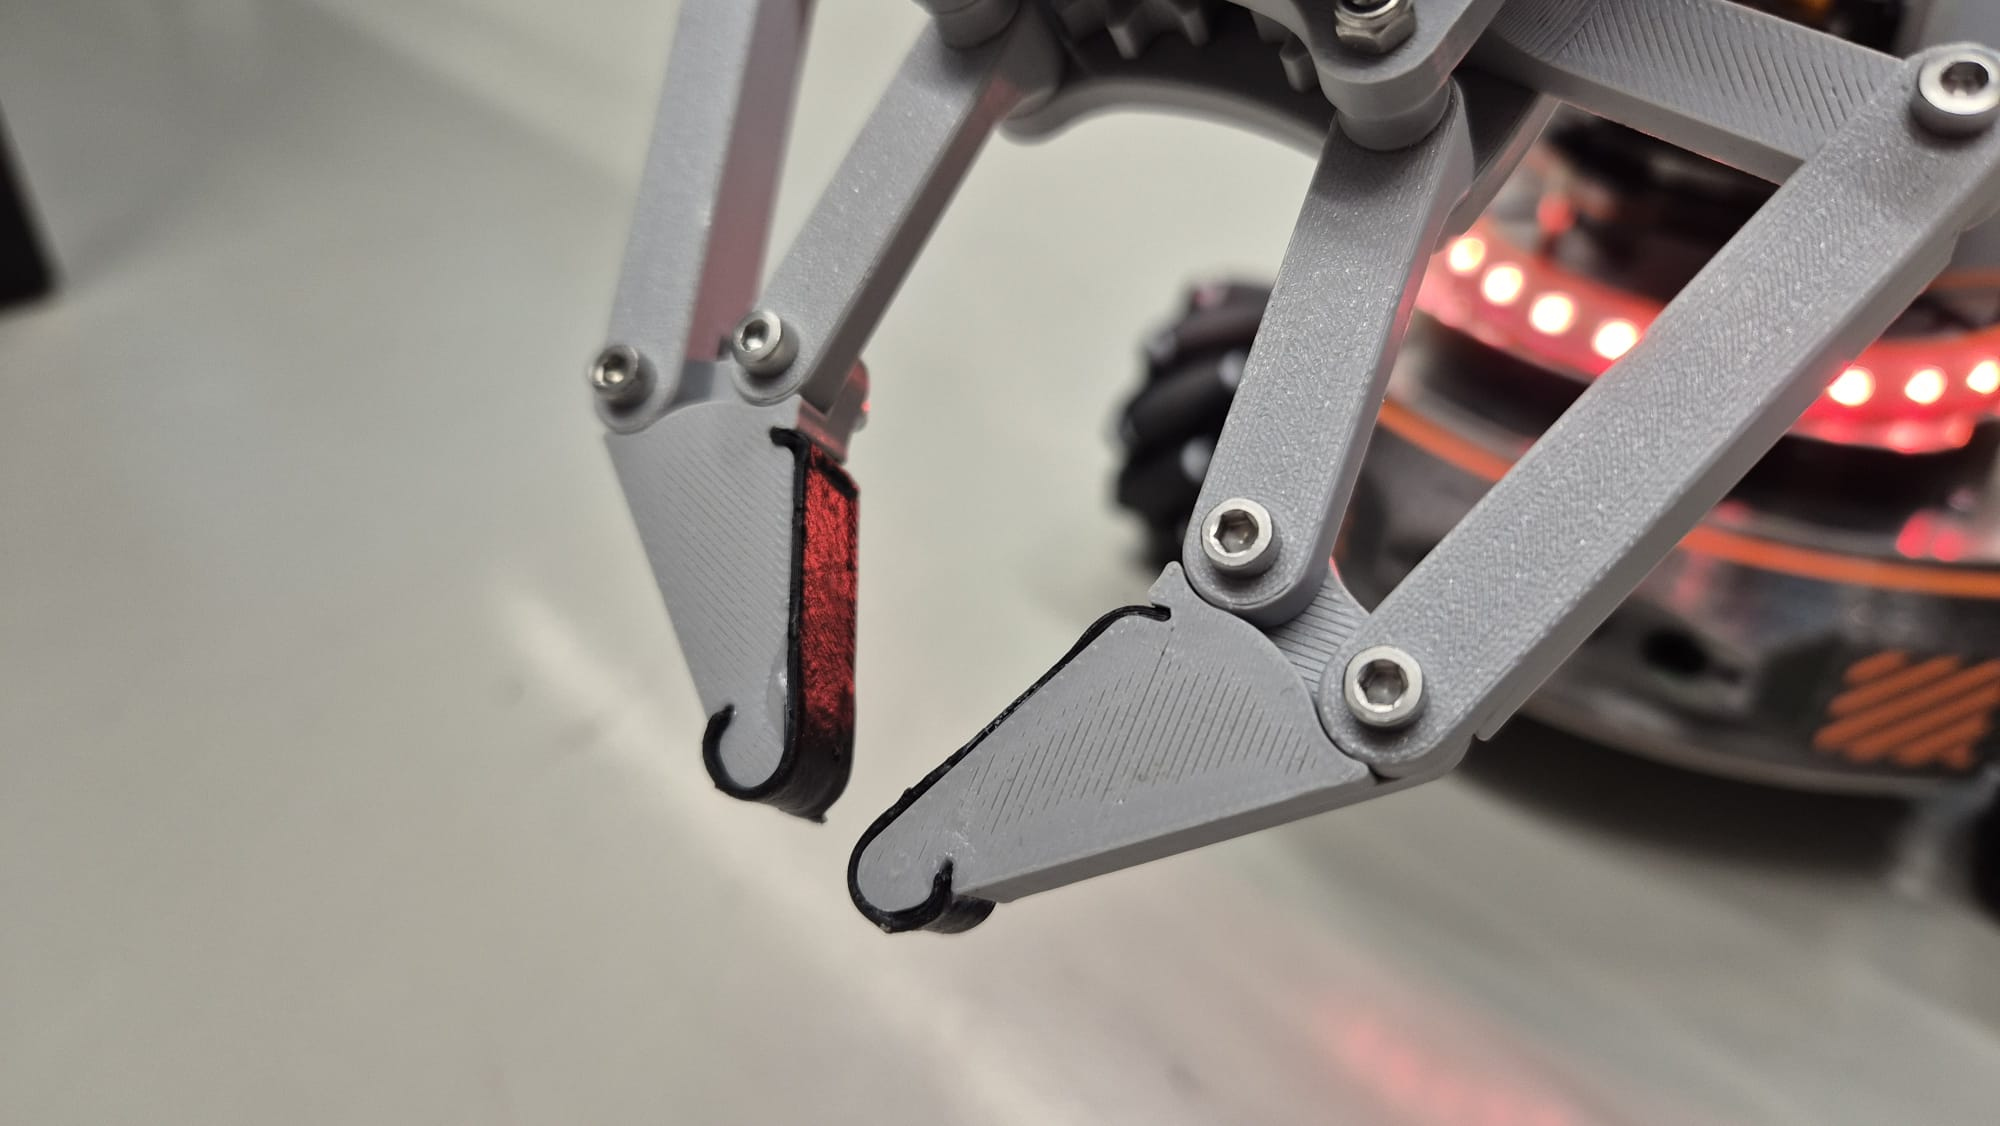
\includegraphics[width=0.99\linewidth]{latex/figures/RubberizedGrippingSurfaces.jpeg}
    \caption{Rubberized gripping surfaces.}
    \label{fig_rubberizedgrippingsurfaces}
    \end{figure}
    \switchcolumn
    \end{paracol}

